Avant la conception du projet il est nécessaire la prise en main du logiciel VLAB et l'utilisation des toolbox disponibles comme le toolbox CAN, Ethernet, LIN et aurix. J'ai d'abord instal\'e l'environement du travail avec les identifiants pour acceder a la reseaux interne de la soci\'et\'e. Deuxièmement, j'ai telecharge les dossiers du travail depuis les servers d'Australie. Apr\`es, j'ai compil\'e du logiciel simple pour tester le microcontr\^oleur (désormais appel\'e \textit{aurix}). Finalement j'ai mod\'elis\'e quelques composants génériques pour tester des autres fonctionalit\'es du VLAB comme les connections des bancs de test, l'envoie de donn\'ees a travers des différents réseaux, entre autres. Le développement de ce projet a \'et\'e divis\'e en 3 parties en fonction de l'évolution du même.

\subsection{First Demo}

Le premier exemple est fait pour tester le logiciel avec une configuration super simple. Il consiste a envoyer une trame CAN et le SWC la reenvoie vers le CANID source. Pour cet exemple une ECU generique a \'et\'e modélisé pour recevoir des trames CAN et LIN. Sur la figure \ref{fig:first-demo-diagram} on peut voir les connections. Malheureusement, cette premiere demo a \'et\'e con\c cue pour \^etre test\'e avec le logiciel CANoe dont nous ne posedons pas la license et SWC n'a pas march\'e comme attendu. Les possibles explications sont las suivantes :

\begin{itemize}
    \item Un protocole inconnu : Même si CANoe utilise le protocole CAN, il envoie peut \^etre d'autres trames d'identification avant le test.
    \item Un SWC peu test\'e : Selon la documentation de ce test, ce SWC n'a pas \'et\'e teste au fond parce que son utilisation ne sera jamais implement\'e, c'est juste un test des logiciels.
\end{itemize}

Quand même, avec ce test j'ai acquis une connaissance basique du fonctionnement des logiciels AUTOSAR ce qui a rendu mon travaille future plus rapide et efficace. Un autre connaissance acquis dans ce partie c'était la partie de modélisation et le modèle de ECU déjà développe sera utilise plus tard.

%En el primer demo para hacer la prise en main de AUTOSAR habia un ejemplo el cual debia funcionar con el programa CANoe. Se intento replicar el comportamiento del CANoe haciendole ingenieria inversa a los codigos. Se encontro el CanId necesario para que el ECU recibiera el frame CAN pero al parecer esto sigue un protocolo mas preciso por parte del programa del demo (CANoe). Decidimos dejarlo aqui porque eso no era productivo para el proyecto pero se aprendio muchisimo de autosar y de la forma en como esta estructurado su stack de comunicacion.

\begin{figure}[!htb]
 \centering
 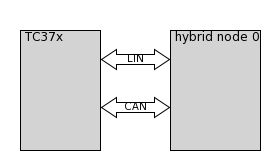
\includegraphics[]{img/first_demo_testbench.png}
 \caption{Premier demo}
 \label{fig:first-demo-diagram}
\end{figure}
%\begin{verbatim}
%/* Appl/GenData/CanIf_Lcfg.c L279 */
%CONST(CanIf_RxPduConfigType, CANIF_CONST) CanIf_RxPduConfig[8] = {  /* PRQA S 1514, 1533 */  /* MD_CSL_ObjectOnlyAccessedOnce */
%    /*Index    RxPduCanId  RxPduMask  UpperPduId                                  RxIndicationFctListIdx   RxPduDlc   MsgType                      
%  { /* 0 */    0x0400u  ,  0x643Fu  , CanNmConf_CanNmRxPdu_CAN_5f8bc0cc_Rx      , 1u               ,       8u         , CANIF_MSG_TYPE_CAN       },
%  { /* 1 */    0x0614u  ,  0x07FFu  , CanTpConf_CanTpRxNPdu_CanTpRxNPdu_e872022a, 2u               ,       8u         , CANIF_MSG_TYPE_NO_FD_CAN },
%  { /* 2 */    0x0610u  ,  0x07FFu  , CanTpConf_CanTpRxNPdu_CanTpRxNPdu_29945216, 2u               ,       8u         , CANIF_MSG_TYPE_NO_FD_CAN },
%  { /* 3 */    0x0501u  ,  0x07FFu  , PduRConf_PduRSrcPdu_PduRSrcPdu_7a86d966   , 3u               ,      64u         , CANIF_MSG_TYPE_CAN       },
%  { /* 4 */    0x0310u  ,  0x07FFu  , PduRConf_PduRSrcPdu_PduRSrcPdu_37e6280b   , 3u               ,       4u         , CANIF_MSG_TYPE_CAN       },
%  { /* 5 */    0x0210u  ,  0x07FFu  , PduRConf_PduRSrcPdu_PduRSrcPdu_9e00b2d3   , 3u               ,       1u         , CANIF_MSG_TYPE_CAN       },
%  { /* 6 */    0x0120u  ,  0x07FFu  , PduRConf_PduRSrcPdu_PduRSrcPdu_01c8980f   , 3u               ,       8u         , CANIF_MSG_TYPE_CAN       },
%  { /* 7 */    0x0110u  ,  0x07FFu  , PduRConf_PduRSrcPdu_PduRSrcPdu_b1d1dd8a   , 3u               ,       6u         , CANIF_MSG_TYPE_CAN       } 
%};
%\end{verbatim}

\subsection{Gateway}

\begin{figure}[!htb]
 \centering
 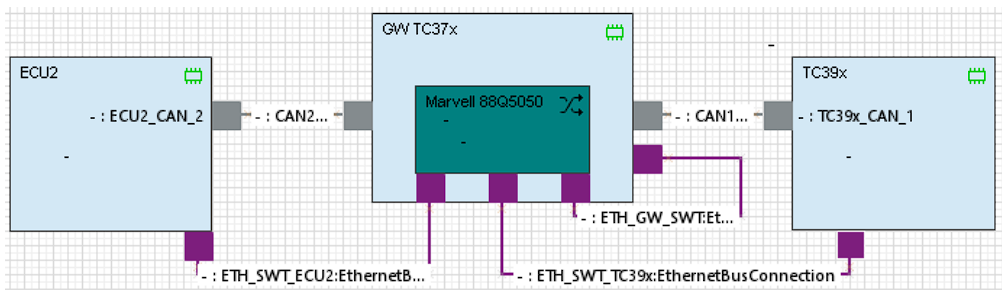
\includegraphics[width=\textwidth]{img/GWDemoConnections.PNG}
 \caption{Gateway Demo Devices}
 \label{fig:devices-diagram}
\end{figure}

Un gateway es un nodo de una red que se comunica con una red exterior, usualmente mas grande. Las ventajas de este gateway es que permite conectar varios protocolos de comunicacion como el Fr, CAN, LIN o ETH, para complementar ECU's que no necesariamente esten programadas para utilizarlos. 

Este gateway en si mismo es una ECU programable con el sistema operativo MICROSAR Classic en el cual podemos preprocesar datos antes de comunicarnos con un protocolo exterior. 

Ademas de esto, este gateway cuenta con un switch ethernet securise que soporta un ancho de banda y velocidades muy altas. Esto permite, por ejemplo, a un sistema de inteligencia artifial de conduccion acceder a una camara de 4k a traves de ethernet (por el ancho de banda grande que este tipo de media necesita) procesar datos y hacer una bien su trabajo, pero al tiempo puede pedir datos o enviar a otra ECU por LIN o CAN sin tener el protocolo fisico integrado. Tambien se pueden recibir muchos datos de internet como estado del trafico o datos de navegacion en tiempo real sin saturar protocolos de comunicacion como el LIN o Fr que tienen muchisimo menos ancho de banda.


\subsection{TC37xEXT}
Al comienzo del proyecto empezamos usando el microcontrolador AURIX TC37x \cite{aurix.tc37x} pero luego leyendo el datasheet del Gateway nos dimos cuenta que en realidad se estaba usando el TC37xEXT \cite{aurix.tc37e} el cual es una version con mas modulos disponibles, entre ellos un modulo CAN y un modulo GETH extras los cuales serian utiles en nuestro proyecto. Otras diferencias se encuentran en la tabla \ref{tab:tc37x_delta}.


% Table generated by Excel2LaTeX from sheet 'Sheet1'
\begin{table}[htbp]
  \centering
    \begin{tabular}{|r||l|l|}
	\hline
	\multirow{2}{*}{Module} & \multicolumn{2}{c|}{Aurix}\\
	\cline{2-3}
	& TC37x & TC37xEXT \\
	\hline \hline
	    RAM & TRAM (cached, non-cached) & EMEM (cached, non-cached) \\
	    \hline
	    CAN interfaces & 2 & 3 \\
	    \hline
	    Camera Interface & not present & CIF \\
	    \hline
	    Gigabit Ethernet Interface & 1 & 2 \\
	    \hline
	    SD interface & not present & present \\
	    \hline
	    eMMC interface & not present & present \\
	    \hline
	\hline
    \end{tabular}
  \caption{TC37x Vs TC37xEXT}
  \label{tab:tc37x_delta}
\end{table}


Para modelisar los microcontroladores se utiliza python2, tomamos los modelos de cada modulo (memorias, mcmcan, cpus, etc) y los unimos a un bus con su respectiva start address y luego lo compilamos. Al final agregamos el nuevo microcontrolador al toolbox ya creado para poder tener todo bien clean.

El siguiente paso fue testear el microcontrolador. Para programar en estos microcontroladores se usa BIFACES, un compilador especial para estas CPU's. Para testear las memorias se escribieron datos y se leyeron luego. Para el modulo CAN y GETH se testearon sus memorias RAM y se enviaron un par de mensajes hacia una ECU externa  y se verificaron. Todo salio bien y pudimos avanzar con el proyecto.

\subsection{Switch Marvell 88Q5050}

Para que el demo arranque nosotros el sw hace ciertas verificaciones de sus componentes como buses de datos funcionales y verifica el correcto comportamiento de ciertos componentes. En este contexto, el switch marvell 88Q5050 juega una papel muy importante en este proceso. El microcontrolador tiene una secuencia muy precisa para verificar el correcto comportamiento del switch, incluyendo leer y escribir registros por el BUS MDIO y descargar todos los registros del switch para luego usarlos. La secuencia de inicializacion esta detallada en el anexo \ref{anexe:switch-init}. Si se enceuntran errores en esta secuencia de inicializacion el sistema operativo no va a inicar los puertos de comunicacion ethernet y por tanto los demos del gateway no van a funcionar de la mejor manera.


Un dato interesante de este switch es que ademas de funcionar como switch ethernet, permite un modo de funcionamiento Distributed Switch Architecture el cual permite que una o varias cpus externas le envien comandos a la cpu del switch para modificar registros dentro del switch o para procesar datos antes de enviarlos o cualquier otra cosa. Este modo de comunicacion da muchisima flexibilidad porque con nuestra ECU podemos controlar el funcionamiento a bajo nivel del switch evitando que sea un componente pasivo y dandole el control al desarrollador de todo lo que quiera hacer con el switch.


Otro problema que nos encontramos realizando esta parte esque el modelo de comunicaciones ethernet del toolbox aurix no permitia protocolos SNAP y el protocolo mencionado arriba es un protocolo SNAP asi que toco agregar el soporte para protocolos SNAP en el modelo propio de aurix. Se testeo luego el comportamiento inical y todo estaba funcionando bien.

Para modelar el switch se utilizo systemC. Se modelo el Switch con base a la informacion fournie por parte del fabricante y se siguio con el proyecto.

\subsection{Use Case 1}

En la figura \ref{fig:block diagram} podemos ver que modulos se comunican con que dispositivo. Para el Use case 1 probamos enviando un mensaje CAN desde la ECU2 con el Id encontrado en el sw de autosar y este funciona ya que envia el mensaje a traves de todo el stack de comunicaciones de autosar pero lastimosamente cuando llega al socket adapter se muere porque los puertos no han sido activados, mala configuracion del switch.

\begin{figure}[!htb]
 \centering
 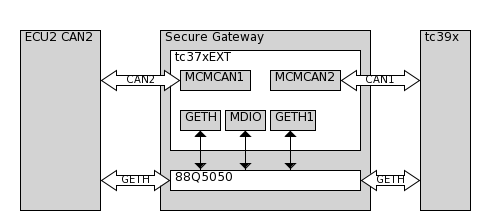
\includegraphics[width=\textwidth]{img/gateway_block_diagram.png}
 \caption{Gateway Block diagram}
 \label{fig:block diagram}
\end{figure}

\begin{figure}[!htb]
 \centering
 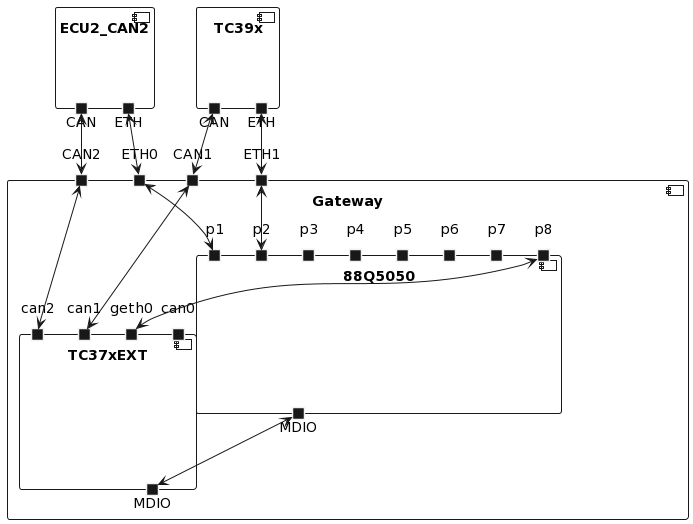
\includegraphics[width=\textwidth]{img/GWConnectionsDiagram.png}
 \caption{Gateway Connections Diagram}
 \label{fig:connections-diagram}
\end{figure}

%Ya con el microcontrolador correcto podemos pasar al demo precargado en microsar tiene 2 USe cases en los que primero se envia algo por CAN y se le hace un forward por eth y viceversa.
%Segun la documentacion del gateway, este gateway esta conectado de la forma mostrada en la figura \ref{fig:connections-diagram}. 

Luego muestras que envias un dato desde CAN con el id que es y que no funcionaba porque patata

\subsection{Use Case 2}

El segundo es uno en el que se envian datos por geth y se reciben por CAN.
No se llego a este caso porque se paso mucho tiempo modelando el switch y analizando el codigo AUTOSAR y modelando el tc37xEXT.
